%%%%%%%%%%%%%%%%%%%%%% section 4%%%%%%%%%%%%%%%%%%%%%
\section{The $M/M/1$ Queuing System}
We now discuss the simplest non-trivial queueing system.  
\subsection{Basics} An $M/M/1/\textrm{GD}/\infty/\infty$ queueing system has exponential inter-arrival times, exponential service times, and a single server. It can be modeled as a birth-death process with
\begin{align*}
\lambda_{j} &= \lambda, \ j=0,1,2,\ldots \\ 
\mu_{0} &= 0 \\
\mu_{j} &= \mu,\  j=1,2,3,\ldots 
\end{align*}
Substituting these rates in (\ref{eq:ssbr}) yields 
$$\pi_{j} = \frac{\lambda^{j} \pi_{0}}{\mu^{j}}=\rho^j \pi_0,$$ where $\rho = \lambda/\mu$ is the \textbf{traffic intensity} of the system. \newpage\noindent 
Since the system has to be in exactly one of the states at any given moment, the sum of all probabilities is 1: $$\pi_{0}+\pi_1 + \pi_2+\cdots = \pi_0(1+\rho+\rho^{2}+\cdots ) = 1.$$
If $0 \leq \rho < 1$, the infinite series converges to $\frac{1}{1-\rho}$ from which we derive $$\pi_{0}\cdot \frac{1}{1-\rho} = 1 \implies \pi_0 = 1-\rho \implies \pi_{j} = \rho^{j} \pi_0 = \rho^j (1-\rho)$$
as the \textbf{steady-state probability of state $j$}.  If $\rho \geq 1$, the infinite series diverges and no steady-state exists. Intuitively, this happens when $\lambda \geq \mu$, that is, if the arrival rate is greater than the service rate, then the state of the system grows without bounds and the queue is never cleared.
\newl From this point on, we assume $\rho < 1$ to guarantee that the steady-state probabilities $\pi_{j}$  exist, from which we can determine several quantities of interest. \par Assuming that the steady state has been reached, it can be shown that $L$, $L_{s}$, and $L_{q}$ are given respectively by:
\begin{align*}
L &= \frac{\lambda}{\mu - \lambda}=\frac{\rho}{1-\rho}\\
L_{s} &= \rho\\
 L_{q} &= \frac{\rho^{2}}{1-\rho}.
 \end{align*}
Using Little's queuing formula, we can also solve for $W$, $W_{s}$, and $W_{q}$ by dividing each of the corresponding $L$ values by~$\lambda$:
\begin{align*}
W &= \frac{1}{\mu - \lambda}\\
W_{s} &= \frac{1}{\mu}\\
W_{q} &= \frac{\lambda}{\mu(\mu-\lambda)}.
 \end{align*}
Notice that, as expected, both $W,W_q\to +\infty$ when $\rho\to 1$. On the other hand, $W_{q}\to 0$ and $W\to \frac{1}{\mu}$ (the \textbf{mean service time}) as $\rho\to 0$.
\begin{Example} (Based on \cite{QS_W}) An average of 10 cars arrive at a single-server drive-in teller every hour. If the average customer is served in 4 minutes, service time for each customer is 4 minutes, and both inter-arrival times and service times are exponential, then: \begin{itemize}[noitemsep]
	\item[(a)] What is the probability that the teller is idle? 
	\item[(b)] Excluding the car that is being served, what is the average number of cars waiting in line at the teller? 
	\item[(c)] What is the average amount of time a drive-in customer spends in the bank parking lot (including time in service)?
	\item[(d)] On average, how many customers per hour will be served by the teller?
\end{itemize}
\textbf{Solution:} by assumption, we are dealing with an $$M/M/1/\textrm{GD}/\infty/\infty$$ queuing system for which $\lambda = 10$ cars/hr and $\mu = 15$ cars/hr, and as such  $\rho = 10/15 = 2/3$.
\begin{itemize}[noitemsep]
	\item[(a)] The teller is idle one third of the time on average because $\pi_{0} = 1 - \rho = 1/3$.
	\item[(b)] There are $L_{q} = \rho^{2}/(1-\rho) = 4/3$ cars waiting in line for the teller. 
	\item[(c)] We know that $L = \lambda/(\mu - \lambda) = 10/(15-10) = 2$, and so $W = L/\lambda = 0.2 \textrm{ hr} = 12 \textrm{ min}$.
	\item[(d)] If the teller were always busy, it would serve an average of $\mu = 15$ customers per hour. From (a), we know that the teller is only busy two-thirds of the time, thus during each hour, the teller serves an average of $15 \cdot 2/3 = 10$ customers. This is reasonable since, in a steady-state, $10$ customers are arriving each hour and $10$ customers must leave the system every hour.
\end{itemize}
\end{Example}
\begin{Example} (Based on \cite{QS_E}) Suppose that all car owners fill up when their tanks are exactly half full.  At the present time, an average of $7.5$ customers arrive every hour at a single-pump gas station. It takes an average of $4$ minutes to fuel a car. Assume that inter-arrival times and service times are both exponential. \begin{itemize}[noitemsep]
	\item[(a)] What are the values of $L$ and $W$ in this scenario? 
	\item[(b)] Suppose that a gas shortage occurs and panic buying takes place. To model this phenomenon, assume that all car owners now purchase gas when their tanks are exactly three-quarters full. Since each car owner is now putting less gas into the tank during each visit to the station, we assume that the average service time has been reduced to $10/3$ minutes. How has panic buying affected the values of $L$ and $W$?
\end{itemize}
\textbf{Solution:} by assumption, we again have an $$M/M/1/\textrm{GD}/\infty/\infty$$ queuing system, with $\lambda = 7.5$ cars/hr and $\mu = 60/4 = 15$ cars/hr.  Thus, $\rho = 7.5/15 = 1/2$.
\begin{enumerate}[noitemsep]
	\item[(a)] By definition, $L = \lambda/(\mu - \lambda) = 7.5/(15-7.5) = 1$ and $W = 1/7.5 \approx 0.13$ hr $=7.8$ min. Hence, in this situation, everything is under control, and long lines appear to be unlikely.
\item[(b)] Under the panic buying scenario,  $\lambda = 2(7.5)=15$ cars/hr as each car owner now fills up twice as often, and $\mu = 60 \cdot 3 /10  = 18$ cars/hr, so $\rho = \lambda/\mu = 5/6$. In that scenario,  
$$ L = \frac{\rho}{1-\rho} = 5 \text{ cars, and } W = \frac{L}{\lambda} = \frac{5}{15} = 20 \text{ min}.$$
Thus, panic buying has more than doubled the wait time in line.
\end{enumerate}
\end{Example}
\newpage\noindent In a $M/M/1$ queueing system, we have $$L=\frac{\rho}{1-\rho}=-1+\frac{1}{1-\rho}, $$ and it is easy to see that $L\to\infty$ as $\rho\to 1$. The $5-$fold increase in $L$ when $\rho$ jumps from $1/2$ to $5/6$ (with accompanying jumps in $W$) illustrate that fact. 
\subsection{Limited Capacity}
In the real world, queues never become infinite -- they are limited due to requirements of {space} and/or {time}, or service operating policy. Such a queuing model falls under the purview of \textbf{finite queues}. \par Finite queue models restrict the number of customers allowed in the service system. Let $N$ represent the maximum allowable number of customers in the system. If the system is at \textbf{capacity}, the arrival of a $(N+1)^{\textrm{th}}$ customer results in a failure to enter the queue -- the customer is assumed balk and depart without seeking service.\newl Finite queues can also be modeled as a birth-death process, but with a slight modification in its parameters:  with these parameters:
\begin{align*}
\lambda_{j} &= \lambda, \ j=0,1,2,\ldots,N-1 \\ 
\lambda_{N} &= 0,\ \mu_{0} = 0 \\
\mu_{j} &= \mu,\  j=1,2,3,\ldots, N 
\end{align*}
The restriction $\lambda_{N} = 0$ is what sets this model apart from the $M/M/1/\infty$. It makes it impossible to reach a state greater than $N$. Because of this restriction, a steady-state always exist because even if $\lambda \geq \mu$, there can never be more than $N$ customers in the system.
\newl Mathematically, this has the effect of replacing the infinite series linking the $\pi_j$'s by a finite geometric series, which always converges: 
$$ \pi_{0}+\pi_1 + +\cdots + \pi_N = \pi_0(1+\rho+\cdots +\rho^{N}) = 1,$$ from which we can derive \begin{align*}\pi_{0}\cdot \frac{1-\rho^{N+1}}{1-\rho} = 1 &\implies \pi_0 = \frac{1-\rho}{1-\rho^{N+1}} \\ &\implies \pi_{j} = \begin{cases}\rho^{j} \frac{1-\rho}{1-\rho^{N+1}} & \text{for $j=0,\ldots,N$} \\ 0 & \text{for $j>N$}\end{cases}\end{align*}
Since $L = \sum^{N}_{j=0} j\cdot \pi_{j}$ (why?), 
$$L = \frac{\rho [1+ N \rho^{N+1} - (N+1) \rho^{N} ]}{(1-\rho)\left(1-\rho^{N+1}\right)} $$
when $\lambda\neq\mu$. \newl As in the $M/M/1/\infty$ queue, $L_{s} = 1 - \pi_{0}$, and $L_{q} = L - L_{s}$.  \newpage\noindent In a finite capacity model, only $\lambda - \lambda \pi_{N} = \lambda\left(1-\pi_{N}\right)$ arrivals per unit time  actually enter the system on average ($\lambda$ arrive, but $\lambda\pi_N$ find the system full). With this fact, 
$$ W = \frac{L}{\lambda\left(1-\pi_{N}\right)}\quad \text{and}\quad W_{q} = \frac{L_{q}}{\lambda\left(1-\pi_{N}\right)}.$$
What does that look like in practice? 
\begin{Example} Consider a one-man barber shop with a total of 10 seats. Assume, as has always been the case so far (but need not be), that inter-arrival times are exponentially distributed with an average of 20 prospective customers arriving each hour at the shop. Those customers who find the shop full do not enter (perhaps they do not like standing). The barber takes an average of 12 minutes to cut each customer's hair; assume that haircut times are also exponentially distributed.
\begin{itemize}[noitemsep]
	\item[(a)] On average, how many haircuts per hour will the barber complete?
	\item[(b)] On average, how much time will be spent in the shop by a customer who enters?
\end{itemize}
\textbf{Solution:} there is not that much to say. Let's dive in!
\begin{itemize}[noitemsep]
	\item[(a)] A fraction $\pi_{10}$ of all arrivals will find the shop full. Thus, an average of $\lambda\left(1-\pi_{10}\right)$ will actually enter the shop each hour.  All entering customers receive a haircut, so the barber will give an average of $\lambda\left(1-\pi_{10}\right)$ haircuts per hour. In this scenario, $N=10$, $\lambda=20$ customers/hr, and $\mu=60/12 = 5 $ customers/hr. Thus $\rho= 20/5 = 4$ and  we have 
	\begin{align*} \pi_{0} &= \frac{1-\rho}{1-\rho^{N+1}} = \frac{1-4}{1-4^{11}}\approx 7.15\times 10^{-7}  \text{ and} \\ \pi_{10} &= 4^{10} \pi_{0} = \frac{3}{4} \text{ (from formula in opposite column)}.\end{align*}
Thus, an average of $20(1 - 3/4)= 5$ customers per hour will receive haircuts. This means that an average of $20 - 5 = 15$ prospective customers per hour will not enter the shop.	
\item[(b)] To determine $W$, we must first compute 
$$L = \frac{4 [1+ (10) 4^{11} - (11) 4^{10} ]}{(1-4)\left(1-4^{11}\right)} = 9.67.$$ 
Using the formulas described above, we obtain 
$$ W = \frac{L}{\lambda\left(1-\pi_{10}\right)} = \frac{9.67}{5} = 1.93 \text{ hr}.$$
This barber shop is crowded -- the barber would be well-advised to hire at least one more barber!
\end{itemize}
\end{Example}
\noindent What \textit{would} be the effect of hiring a second barber? In order to answer this question, we will study $M/M/c$ queueing systems.   
%%%%%%%%%%%_________Section 5____________%%%%%%%%%%%%%%%%%%%%
\begin{figure*}[!t]
\centering
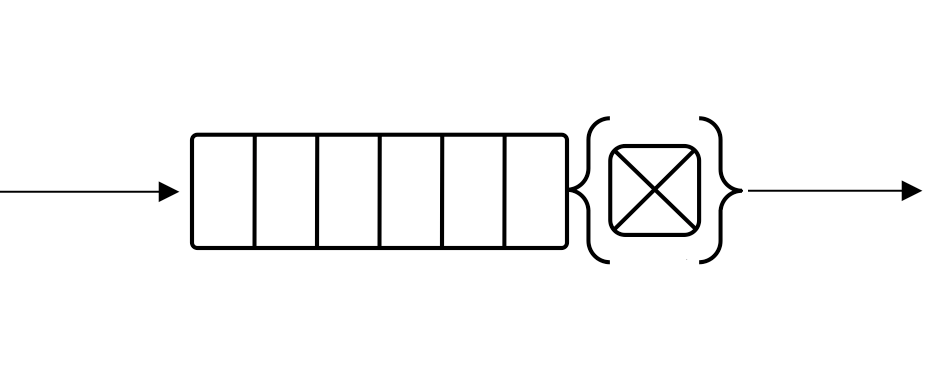
\includegraphics[width=0.45\textwidth]{Images/MM12.png}\qquad\qquad 
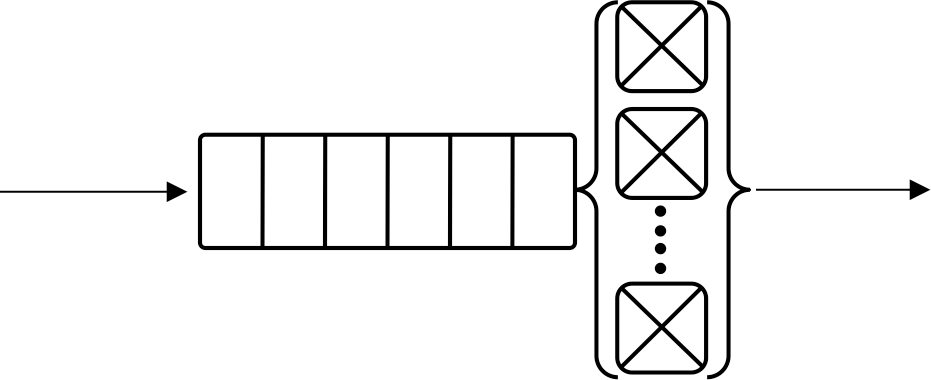
\includegraphics[width=0.45\textwidth]{Images/MMc.png}\\
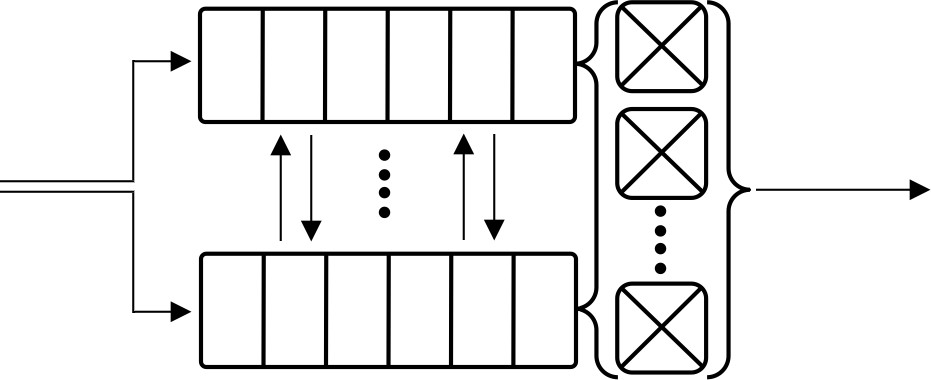
\includegraphics[width=0.45\textwidth]{Images/Tandem.png}
\caption{\small Schematics of various queueing systems ($M/M/1$, $M/M/c$, tandem); customers arrive from the left, enter the queue and progress through it until they are served, at which point the exit the queue.}\label{fig:MM}\hrule
\end{figure*}\afterpage{\FloatBarrier}
